\documentclass[10pt]{article}
\usepackage{tmlr}
% \usepackage[accepted]{tmlr}
% \usepackage[preprint]{tmlr}

%%%%% NEW MATH DEFINITIONS %%%%%

\usepackage{amsmath,amsfonts,bm}

% Mark sections of captions for referring to divisions of figures
\newcommand{\figleft}{{\em (Left)}}
\newcommand{\figcenter}{{\em (Center)}}
\newcommand{\figright}{{\em (Right)}}
\newcommand{\figtop}{{\em (Top)}}
\newcommand{\figbottom}{{\em (Bottom)}}
\newcommand{\captiona}{{\em (a)}}
\newcommand{\captionb}{{\em (b)}}
\newcommand{\captionc}{{\em (c)}}
\newcommand{\captiond}{{\em (d)}}

% Highlight a newly defined term
\newcommand{\newterm}[1]{{\bf #1}}


% Figure reference, lower-case.
\def\figref#1{figure~\ref{#1}}
% Figure reference, capital. For start of sentence
\def\Figref#1{Figure~\ref{#1}}
\def\twofigref#1#2{figures \ref{#1} and \ref{#2}}
\def\quadfigref#1#2#3#4{figures \ref{#1}, \ref{#2}, \ref{#3} and \ref{#4}}
% Section reference, lower-case.
\def\secref#1{section~\ref{#1}}
% Section reference, capital.
\def\Secref#1{Section~\ref{#1}}
% Reference to two sections.
\def\twosecrefs#1#2{sections \ref{#1} and \ref{#2}}
% Reference to three sections.
\def\secrefs#1#2#3{sections \ref{#1}, \ref{#2} and \ref{#3}}
% Reference to an equation, lower-case.
\def\eqref#1{equation~\ref{#1}}
% Reference to an equation, upper case
\def\Eqref#1{Equation~\ref{#1}}
% A raw reference to an equation---avoid using if possible
\def\plaineqref#1{\ref{#1}}
% Reference to a chapter, lower-case.
\def\chapref#1{chapter~\ref{#1}}
% Reference to an equation, upper case.
\def\Chapref#1{Chapter~\ref{#1}}
% Reference to a range of chapters
\def\rangechapref#1#2{chapters\ref{#1}--\ref{#2}}
% Reference to an algorithm, lower-case.
\def\algref#1{algorithm~\ref{#1}}
% Reference to an algorithm, upper case.
\def\Algref#1{Algorithm~\ref{#1}}
\def\twoalgref#1#2{algorithms \ref{#1} and \ref{#2}}
\def\Twoalgref#1#2{Algorithms \ref{#1} and \ref{#2}}
% Reference to a part, lower case
\def\partref#1{part~\ref{#1}}
% Reference to a part, upper case
\def\Partref#1{Part~\ref{#1}}
\def\twopartref#1#2{parts \ref{#1} and \ref{#2}}

\def\ceil#1{\lceil #1 \rceil}
\def\floor#1{\lfloor #1 \rfloor}
\def\1{\bm{1}}
\newcommand{\train}{\mathcal{D}}
\newcommand{\valid}{\mathcal{D_{\mathrm{valid}}}}
\newcommand{\test}{\mathcal{D_{\mathrm{test}}}}

\def\eps{{\epsilon}}


% Random variables
\def\reta{{\textnormal{$\eta$}}}
\def\ra{{\textnormal{a}}}
\def\rb{{\textnormal{b}}}
\def\rc{{\textnormal{c}}}
\def\rd{{\textnormal{d}}}
\def\re{{\textnormal{e}}}
\def\rf{{\textnormal{f}}}
\def\rg{{\textnormal{g}}}
\def\rh{{\textnormal{h}}}
\def\ri{{\textnormal{i}}}
\def\rj{{\textnormal{j}}}
\def\rk{{\textnormal{k}}}
\def\rl{{\textnormal{l}}}
% rm is already a command, just don't name any random variables m
\def\rn{{\textnormal{n}}}
\def\ro{{\textnormal{o}}}
\def\rp{{\textnormal{p}}}
\def\rq{{\textnormal{q}}}
\def\rr{{\textnormal{r}}}
\def\rs{{\textnormal{s}}}
\def\rt{{\textnormal{t}}}
\def\ru{{\textnormal{u}}}
\def\rv{{\textnormal{v}}}
\def\rw{{\textnormal{w}}}
\def\rx{{\textnormal{x}}}
\def\ry{{\textnormal{y}}}
\def\rz{{\textnormal{z}}}

% Random vectors
\def\rvepsilon{{\mathbf{\epsilon}}}
\def\rvtheta{{\mathbf{\theta}}}
\def\rva{{\mathbf{a}}}
\def\rvb{{\mathbf{b}}}
\def\rvc{{\mathbf{c}}}
\def\rvd{{\mathbf{d}}}
\def\rve{{\mathbf{e}}}
\def\rvf{{\mathbf{f}}}
\def\rvg{{\mathbf{g}}}
\def\rvh{{\mathbf{h}}}
\def\rvu{{\mathbf{i}}}
\def\rvj{{\mathbf{j}}}
\def\rvk{{\mathbf{k}}}
\def\rvl{{\mathbf{l}}}
\def\rvm{{\mathbf{m}}}
\def\rvn{{\mathbf{n}}}
\def\rvo{{\mathbf{o}}}
\def\rvp{{\mathbf{p}}}
\def\rvq{{\mathbf{q}}}
\def\rvr{{\mathbf{r}}}
\def\rvs{{\mathbf{s}}}
\def\rvt{{\mathbf{t}}}
\def\rvu{{\mathbf{u}}}
\def\rvv{{\mathbf{v}}}
\def\rvw{{\mathbf{w}}}
\def\rvx{{\mathbf{x}}}
\def\rvy{{\mathbf{y}}}
\def\rvz{{\mathbf{z}}}

% Elements of random vectors
\def\erva{{\textnormal{a}}}
\def\ervb{{\textnormal{b}}}
\def\ervc{{\textnormal{c}}}
\def\ervd{{\textnormal{d}}}
\def\erve{{\textnormal{e}}}
\def\ervf{{\textnormal{f}}}
\def\ervg{{\textnormal{g}}}
\def\ervh{{\textnormal{h}}}
\def\ervi{{\textnormal{i}}}
\def\ervj{{\textnormal{j}}}
\def\ervk{{\textnormal{k}}}
\def\ervl{{\textnormal{l}}}
\def\ervm{{\textnormal{m}}}
\def\ervn{{\textnormal{n}}}
\def\ervo{{\textnormal{o}}}
\def\ervp{{\textnormal{p}}}
\def\ervq{{\textnormal{q}}}
\def\ervr{{\textnormal{r}}}
\def\ervs{{\textnormal{s}}}
\def\ervt{{\textnormal{t}}}
\def\ervu{{\textnormal{u}}}
\def\ervv{{\textnormal{v}}}
\def\ervw{{\textnormal{w}}}
\def\ervx{{\textnormal{x}}}
\def\ervy{{\textnormal{y}}}
\def\ervz{{\textnormal{z}}}

% Random matrices
\def\rmA{{\mathbf{A}}}
\def\rmB{{\mathbf{B}}}
\def\rmC{{\mathbf{C}}}
\def\rmD{{\mathbf{D}}}
\def\rmE{{\mathbf{E}}}
\def\rmF{{\mathbf{F}}}
\def\rmG{{\mathbf{G}}}
\def\rmH{{\mathbf{H}}}
\def\rmI{{\mathbf{I}}}
\def\rmJ{{\mathbf{J}}}
\def\rmK{{\mathbf{K}}}
\def\rmL{{\mathbf{L}}}
\def\rmM{{\mathbf{M}}}
\def\rmN{{\mathbf{N}}}
\def\rmO{{\mathbf{O}}}
\def\rmP{{\mathbf{P}}}
\def\rmQ{{\mathbf{Q}}}
\def\rmR{{\mathbf{R}}}
\def\rmS{{\mathbf{S}}}
\def\rmT{{\mathbf{T}}}
\def\rmU{{\mathbf{U}}}
\def\rmV{{\mathbf{V}}}
\def\rmW{{\mathbf{W}}}
\def\rmX{{\mathbf{X}}}
\def\rmY{{\mathbf{Y}}}
\def\rmZ{{\mathbf{Z}}}

% Elements of random matrices
\def\ermA{{\textnormal{A}}}
\def\ermB{{\textnormal{B}}}
\def\ermC{{\textnormal{C}}}
\def\ermD{{\textnormal{D}}}
\def\ermE{{\textnormal{E}}}
\def\ermF{{\textnormal{F}}}
\def\ermG{{\textnormal{G}}}
\def\ermH{{\textnormal{H}}}
\def\ermI{{\textnormal{I}}}
\def\ermJ{{\textnormal{J}}}
\def\ermK{{\textnormal{K}}}
\def\ermL{{\textnormal{L}}}
\def\ermM{{\textnormal{M}}}
\def\ermN{{\textnormal{N}}}
\def\ermO{{\textnormal{O}}}
\def\ermP{{\textnormal{P}}}
\def\ermQ{{\textnormal{Q}}}
\def\ermR{{\textnormal{R}}}
\def\ermS{{\textnormal{S}}}
\def\ermT{{\textnormal{T}}}
\def\ermU{{\textnormal{U}}}
\def\ermV{{\textnormal{V}}}
\def\ermW{{\textnormal{W}}}
\def\ermX{{\textnormal{X}}}
\def\ermY{{\textnormal{Y}}}
\def\ermZ{{\textnormal{Z}}}

% Vectors
\def\vzero{{\bm{0}}}
\def\vone{{\bm{1}}}
\def\vmu{{\bm{\mu}}}
\def\vtheta{{\bm{\theta}}}
\def\va{{\bm{a}}}
\def\vb{{\bm{b}}}
\def\vc{{\bm{c}}}
\def\vd{{\bm{d}}}
\def\ve{{\bm{e}}}
\def\vf{{\bm{f}}}
\def\vg{{\bm{g}}}
\def\vh{{\bm{h}}}
\def\vi{{\bm{i}}}
\def\vj{{\bm{j}}}
\def\vk{{\bm{k}}}
\def\vl{{\bm{l}}}
\def\vm{{\bm{m}}}
\def\vn{{\bm{n}}}
\def\vo{{\bm{o}}}
\def\vp{{\bm{p}}}
\def\vq{{\bm{q}}}
\def\vr{{\bm{r}}}
\def\vs{{\bm{s}}}
\def\vt{{\bm{t}}}
\def\vu{{\bm{u}}}
\def\vv{{\bm{v}}}
\def\vw{{\bm{w}}}
\def\vx{{\bm{x}}}
\def\vy{{\bm{y}}}
\def\vz{{\bm{z}}}

% Elements of vectors
\def\evalpha{{\alpha}}
\def\evbeta{{\beta}}
\def\evepsilon{{\epsilon}}
\def\evlambda{{\lambda}}
\def\evomega{{\omega}}
\def\evmu{{\mu}}
\def\evpsi{{\psi}}
\def\evsigma{{\sigma}}
\def\evtheta{{\theta}}
\def\eva{{a}}
\def\evb{{b}}
\def\evc{{c}}
\def\evd{{d}}
\def\eve{{e}}
\def\evf{{f}}
\def\evg{{g}}
\def\evh{{h}}
\def\evi{{i}}
\def\evj{{j}}
\def\evk{{k}}
\def\evl{{l}}
\def\evm{{m}}
\def\evn{{n}}
\def\evo{{o}}
\def\evp{{p}}
\def\evq{{q}}
\def\evr{{r}}
\def\evs{{s}}
\def\evt{{t}}
\def\evu{{u}}
\def\evv{{v}}
\def\evw{{w}}
\def\evx{{x}}
\def\evy{{y}}
\def\evz{{z}}

% Matrix
\def\mA{{\bm{A}}}
\def\mB{{\bm{B}}}
\def\mC{{\bm{C}}}
\def\mD{{\bm{D}}}
\def\mE{{\bm{E}}}
\def\mF{{\bm{F}}}
\def\mG{{\bm{G}}}
\def\mH{{\bm{H}}}
\def\mI{{\bm{I}}}
\def\mJ{{\bm{J}}}
\def\mK{{\bm{K}}}
\def\mL{{\bm{L}}}
\def\mM{{\bm{M}}}
\def\mN{{\bm{N}}}
\def\mO{{\bm{O}}}
\def\mP{{\bm{P}}}
\def\mQ{{\bm{Q}}}
\def\mR{{\bm{R}}}
\def\mS{{\bm{S}}}
\def\mT{{\bm{T}}}
\def\mU{{\bm{U}}}
\def\mV{{\bm{V}}}
\def\mW{{\bm{W}}}
\def\mX{{\bm{X}}}
\def\mY{{\bm{Y}}}
\def\mZ{{\bm{Z}}}
\def\mBeta{{\bm{\beta}}}
\def\mPhi{{\bm{\Phi}}}
\def\mLambda{{\bm{\Lambda}}}
\def\mSigma{{\bm{\Sigma}}}

% Tensor
\DeclareMathAlphabet{\mathsfit}{\encodingdefault}{\sfdefault}{m}{sl}
\SetMathAlphabet{\mathsfit}{bold}{\encodingdefault}{\sfdefault}{bx}{n}
\newcommand{\tens}[1]{\bm{\mathsfit{#1}}}
\def\tA{{\tens{A}}}
\def\tB{{\tens{B}}}
\def\tC{{\tens{C}}}
\def\tD{{\tens{D}}}
\def\tE{{\tens{E}}}
\def\tF{{\tens{F}}}
\def\tG{{\tens{G}}}
\def\tH{{\tens{H}}}
\def\tI{{\tens{I}}}
\def\tJ{{\tens{J}}}
\def\tK{{\tens{K}}}
\def\tL{{\tens{L}}}
\def\tM{{\tens{M}}}
\def\tN{{\tens{N}}}
\def\tO{{\tens{O}}}
\def\tP{{\tens{P}}}
\def\tQ{{\tens{Q}}}
\def\tR{{\tens{R}}}
\def\tS{{\tens{S}}}
\def\tT{{\tens{T}}}
\def\tU{{\tens{U}}}
\def\tV{{\tens{V}}}
\def\tW{{\tens{W}}}
\def\tX{{\tens{X}}}
\def\tY{{\tens{Y}}}
\def\tZ{{\tens{Z}}}


% Graph
\def\gA{{\mathcal{A}}}
\def\gB{{\mathcal{B}}}
\def\gC{{\mathcal{C}}}
\def\gD{{\mathcal{D}}}
\def\gE{{\mathcal{E}}}
\def\gF{{\mathcal{F}}}
\def\gG{{\mathcal{G}}}
\def\gH{{\mathcal{H}}}
\def\gI{{\mathcal{I}}}
\def\gJ{{\mathcal{J}}}
\def\gK{{\mathcal{K}}}
\def\gL{{\mathcal{L}}}
\def\gM{{\mathcal{M}}}
\def\gN{{\mathcal{N}}}
\def\gO{{\mathcal{O}}}
\def\gP{{\mathcal{P}}}
\def\gQ{{\mathcal{Q}}}
\def\gR{{\mathcal{R}}}
\def\gS{{\mathcal{S}}}
\def\gT{{\mathcal{T}}}
\def\gU{{\mathcal{U}}}
\def\gV{{\mathcal{V}}}
\def\gW{{\mathcal{W}}}
\def\gX{{\mathcal{X}}}
\def\gY{{\mathcal{Y}}}
\def\gZ{{\mathcal{Z}}}

% Sets
\def\sA{{\mathbb{A}}}
\def\sB{{\mathbb{B}}}
\def\sC{{\mathbb{C}}}
\def\sD{{\mathbb{D}}}
% Don't use a set called E, because this would be the same as our symbol
% for expectation.
\def\sF{{\mathbb{F}}}
\def\sG{{\mathbb{G}}}
\def\sH{{\mathbb{H}}}
\def\sI{{\mathbb{I}}}
\def\sJ{{\mathbb{J}}}
\def\sK{{\mathbb{K}}}
\def\sL{{\mathbb{L}}}
\def\sM{{\mathbb{M}}}
\def\sN{{\mathbb{N}}}
\def\sO{{\mathbb{O}}}
\def\sP{{\mathbb{P}}}
\def\sQ{{\mathbb{Q}}}
\def\sR{{\mathbb{R}}}
\def\sS{{\mathbb{S}}}
\def\sT{{\mathbb{T}}}
\def\sU{{\mathbb{U}}}
\def\sV{{\mathbb{V}}}
\def\sW{{\mathbb{W}}}
\def\sX{{\mathbb{X}}}
\def\sY{{\mathbb{Y}}}
\def\sZ{{\mathbb{Z}}}

% Entries of a matrix
\def\emLambda{{\Lambda}}
\def\emA{{A}}
\def\emB{{B}}
\def\emC{{C}}
\def\emD{{D}}
\def\emE{{E}}
\def\emF{{F}}
\def\emG{{G}}
\def\emH{{H}}
\def\emI{{I}}
\def\emJ{{J}}
\def\emK{{K}}
\def\emL{{L}}
\def\emM{{M}}
\def\emN{{N}}
\def\emO{{O}}
\def\emP{{P}}
\def\emQ{{Q}}
\def\emR{{R}}
\def\emS{{S}}
\def\emT{{T}}
\def\emU{{U}}
\def\emV{{V}}
\def\emW{{W}}
\def\emX{{X}}
\def\emY{{Y}}
\def\emZ{{Z}}
\def\emSigma{{\Sigma}}

% entries of a tensor
% Same font as tensor, without \bm wrapper
\newcommand{\etens}[1]{\mathsfit{#1}}
\def\etLambda{{\etens{\Lambda}}}
\def\etA{{\etens{A}}}
\def\etB{{\etens{B}}}
\def\etC{{\etens{C}}}
\def\etD{{\etens{D}}}
\def\etE{{\etens{E}}}
\def\etF{{\etens{F}}}
\def\etG{{\etens{G}}}
\def\etH{{\etens{H}}}
\def\etI{{\etens{I}}}
\def\etJ{{\etens{J}}}
\def\etK{{\etens{K}}}
\def\etL{{\etens{L}}}
\def\etM{{\etens{M}}}
\def\etN{{\etens{N}}}
\def\etO{{\etens{O}}}
\def\etP{{\etens{P}}}
\def\etQ{{\etens{Q}}}
\def\etR{{\etens{R}}}
\def\etS{{\etens{S}}}
\def\etT{{\etens{T}}}
\def\etU{{\etens{U}}}
\def\etV{{\etens{V}}}
\def\etW{{\etens{W}}}
\def\etX{{\etens{X}}}
\def\etY{{\etens{Y}}}
\def\etZ{{\etens{Z}}}

% The true underlying data generating distribution
\newcommand{\pdata}{p_{\rm{data}}}
% The empirical distribution defined by the training set
\newcommand{\ptrain}{\hat{p}_{\rm{data}}}
\newcommand{\Ptrain}{\hat{P}_{\rm{data}}}
% The model distribution
\newcommand{\pmodel}{p_{\rm{model}}}
\newcommand{\Pmodel}{P_{\rm{model}}}
\newcommand{\ptildemodel}{\tilde{p}_{\rm{model}}}
% Stochastic autoencoder distributions
\newcommand{\pencode}{p_{\rm{encoder}}}
\newcommand{\pdecode}{p_{\rm{decoder}}}
\newcommand{\precons}{p_{\rm{reconstruct}}}

\newcommand{\laplace}{\mathrm{Laplace}} % Laplace distribution

\newcommand{\E}{\mathbb{E}}
\newcommand{\Ls}{\mathcal{L}}
\newcommand{\R}{\mathbb{R}}
\newcommand{\emp}{\tilde{p}}
\newcommand{\lr}{\alpha}
\newcommand{\reg}{\lambda}
\newcommand{\rect}{\mathrm{rectifier}}
\newcommand{\softmax}{\mathrm{softmax}}
\newcommand{\sigmoid}{\sigma}
\newcommand{\softplus}{\zeta}
\newcommand{\KL}{D_{\mathrm{KL}}}
\newcommand{\Var}{\mathrm{Var}}
\newcommand{\standarderror}{\mathrm{SE}}
\newcommand{\Cov}{\mathrm{Cov}}
% Wolfram Mathworld says $L^2$ is for function spaces and $\ell^2$ is for vectors
% But then they seem to use $L^2$ for vectors throughout the site, and so does
% wikipedia.
\newcommand{\normlzero}{L^0}
\newcommand{\normlone}{L^1}
\newcommand{\normltwo}{L^2}
\newcommand{\normlp}{L^p}
\newcommand{\normmax}{L^\infty}

\newcommand{\parents}{Pa} % See usage in notation.tex. Chosen to match Daphne's book.

\DeclareMathOperator*{\argmax}{arg\,max}
\DeclareMathOperator*{\argmin}{arg\,min}

\DeclareMathOperator{\sign}{sign}
\DeclareMathOperator{\Tr}{Tr}
\let\ab\allowbreak


\usepackage{hyperref}
\usepackage{url}
\usepackage{amsmath,amssymb,amsthm}
\usepackage{booktabs}
\usepackage{graphicx}
\usepackage{xcolor}
\usepackage{multirow}
\usepackage[capitalise,noabbrev]{cleveref}

\newtheorem{theorem}{Theorem}
\newtheorem{proposition}{Proposition}
\newtheorem{lemma}{Lemma}
\newtheorem{corollary}{Corollary}
\theoremstyle{definition}
\newtheorem{definition}{Definition}
\newtheorem{assumption}{Assumption}
\newtheorem{observation}{Observation}
\theoremstyle{remark}
\newtheorem{remark}{Remark}
\crefname{assumption}{Assumption}{Assumptions}
\crefname{observation}{Observation}{Observations}

\newcommand{\fifo}{\textup{\textsc{fifo}}}
\newcommand{\full}{\textup{\textsc{reset}}}
\newcommand{\half}{\textup{\textsc{half}}}
\newcommand{\hedge}{\textup{\textsc{hedge}}}
\newcommand{\ctx}{\mathcal{C}}

\title{Error-Driven Context Resets Are a Tail Risk\\for Tabular In-Context Learners on Data Streams}

\author{\name Anonymous authors \\
      \addr Paper under double-blind review}

\def\month{MM}
\def\year{YYYY}
\def\openreview{\url{https://openreview.net/forum?id=XXXX}}

\begin{document}

\maketitle

\begin{abstract}
Tabular foundation models (TFMs) such as TabPFN, TabICL and TabDPT predict from a context of labelled rows without
gradient updates, which makes them attractive for data streams: keeping the most recent rows in the context (FIFO) is
already a form of adaptation. A long line of stream-learning work adds an error-driven drift detector that, on an
alarm, discards the past. We ask whether this practice transfers to in-context learners. On 39 real streams from 19
independent sources and 42 synthetic streams, with eight detectors, three reset actions and three TFMs, we find that a
full context reset is a \emph{tail risk}: averaged over detectors it loses 26--31 accuracy points on the worst source
while gaining at most 5--6 on the best, and 87--88\% of the single resets that change the outcome on real streams are
net losses. Averaged over sources the effect is not significant after correction for multiple testing, so the
practice is neither uniformly harmful nor useful; its risk sits in the tail. Two facts explain the asymmetry. Under a
FIFO budget, the effect of a reset is confined to the next $\lceil M/B\rceil-1$ batches (we prove this and use it for
exact per-reset accounting), so the window already forgets and leaves a reset little to gain; trained incremental
learners, which never forget, gain from the same resets (+1.8 and +7.3 points on average). We then show that hedging
the reset context against the FIFO context with exponential weights removes the tail at almost no cost: we prove a
log-loss guarantee of at most $\ln 2/\eta$ per detection relative to FIFO, and empirically the worst source improves to
about $-2$ points while 90\% of the best-source gain and the synthetic gains are kept. The findings hold across
backbones, backbone seeds, context budgets and hedge hyperparameters.
\end{abstract}

% ---------------------------------------------------------------------------------------------------------------------
\section{Introduction}
\label{sec:intro}
\begin{figure}[t]
\centering
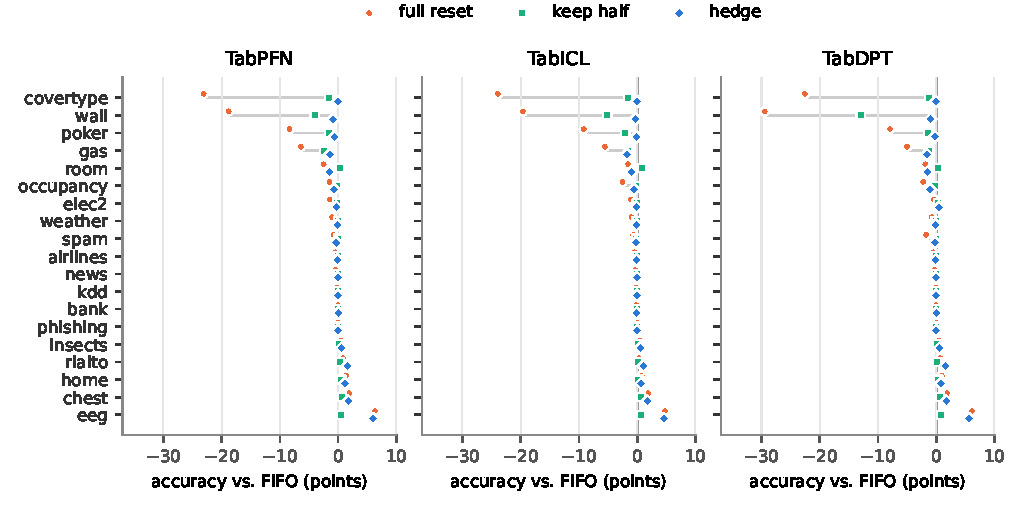
\includegraphics[width=\linewidth]{figs/fig_sources.pdf}
\caption{Effect of the three actions on detection, per real source and averaged over the eight detectors, as accuracy
minus FIFO with the same TFM ($M=1000$). A full reset (orange) loses heavily on a few sources (covertype, wall, poker,
gas) and gains on a few others (eeg, chest, home); hedging against FIFO (blue) removes the losses and keeps the gains.
Sources are ordered by the full-reset effect on TabPFN.}
\label{fig:sources}
\end{figure}


Tabular foundation models are transformers pre-trained on synthetic tasks that solve a new classification problem
in a single forward pass over a \emph{context} of labelled rows \citep{muller2022transformers,hollmann2023tabpfn,
hollmann2025tabpfn,qu2025tabicl,ma2024tabdpt}. On a data stream, the natural way to use such a model is to keep the
most recent $M$ labelled rows as its context and to predict each incoming batch from them. The model is frozen, so
the only thing that adapts is the context, and a first-in-first-out (FIFO) window already forgets old concepts at a
fixed rate.

Classical stream learning adapts in a different way. A learner is trained incrementally, and a drift detector
monitors its error rate; when the detector fires, the learner is reset and retrained on recent data
\citep{gama2004ddm,baena2006eddm,bifet2007adwin,frias2015hddm,pesaranghader2016fhddm,raab2020kswin}. This
detect-and-reset pattern is the default in surveys and libraries \citep{gama2014survey,lu2019survey,montiel2021river}.
For an in-context learner its analogue is simple: on an alarm, empty the context and refill it from the latest labelled
batch. It is tempting to bolt this onto a TFM, and doing so costs nothing to implement. We ask whether it should be
done.

We run the experiment at scale (\cref{sec:setup}): 81 streams (39 real ones from 19 independent sources and 42
synthetic ones), eight error-driven detectors with their default parameters, three actions on detection (full reset,
keep half of the window, and a hedge described below), three TFMs (TabPFN v2, TabICL, TabDPT), three backbone seeds,
three context budgets, and two trained incremental learners for contrast. Every comparison is against the same model
with a FIFO window, and every test treats the 19 real sources, not the 39 streams, as the independent units. Three
observations stand out (\cref{fig:sources}).

\begin{observation}[Resets carry a heavy left tail]
\label{obs:tail}
Averaged over the eight detectors, a full reset loses 26.2, 26.5 and 31.1 accuracy points against FIFO on the worst
real source for TabPFN, TabICL and TabDPT, and gains at most 6.3, 4.8 and 6.1 points on the best. Of the single resets
that change the accuracy of the batches they affect, 87--88\% are net losses on real streams.
\end{observation}

\begin{observation}[The average hides the tail]
\label{obs:average}
Over the 19 real sources the mean effect of a full reset is negative for every detector and backbone, but no detector
is significant after Holm correction, and resets help on several sources (eeg, chest, home). On synthetic streams with
abrupt, recurring concepts resets help by about 8 points.
\end{observation}

\begin{observation}[A FIFO window leaves a reset little to gain]
\label{obs:fifo}
The same detectors on trained learners that never forget gain on average (Hoeffding tree $+1.8$, Gaussian naive
Bayes $+7.3$ points), where TabPFN loses ($-2.8$). On the sources where resets help, they help the trained learners
several times more (eeg: $+28.5$ and $+39.2$ against $+6.3$). For TabPFN the best-source gain grows with the context budget (4.4, 6.3 and 7.7 points for
$M=500,1000,2000$).
\end{observation}

These observations reframe the question. A detector is useful when it fires on a real change and costly when it fires
on noise; a FIFO window already captures most of the benefit of the first case, while a reset pays the full cost of the
second. The practical question is therefore not whether drift detection is good or bad for TFMs, but

\begin{center}
\fbox{\parbox{0.86\linewidth}{\centering\emph{How can an in-context learner on a stream act on a drift alarm without
exposing itself to the tail risk of a false one?}}}
\end{center}

\begin{remark}
We do not propose a new detector or a new stream learner, and we do not claim state-of-the-art accuracy. Our objective
is to establish, with controlled comparisons and source-level statistics, what error-driven resets do to tabular
in-context learners, why, and which minimal change makes them safe to use.
\end{remark}

Our answer is to keep the FIFO context alive next to the reset one and to mix their predictions with exponential
weights on their recent log-loss \citep{vovk1990aggregating,cesabianchi2006prediction}. A false alarm then costs at
most a constant, while a real change is followed within a few batches.

\paragraph{Contributions.}
\begin{enumerate}
\item \textbf{A protocol with exact accounting.} We show that under a FIFO budget a reset changes the context of at
  most $\lceil M/B\rceil-1$ batches (\cref{prop:memory}), so the effect of each single reset can be measured exactly
  and the total effect decomposes into per-reset effects.
\item \textbf{A large controlled evaluation.} Eight detectors $\times$ three actions $\times$ three TFMs on 81 streams,
  with backbone seeds, context budgets and two trained learners, and tests clustered by source
  (\cref{sec:results}). Code, streams and all cached predictions are released.
\item \textbf{A finding and its mechanism.} Error-driven resets are a tail risk for TFMs, not a uniform loss
  (\cref{obs:tail,obs:average}); a FIFO window absorbs most of what a reset could gain (\cref{obs:fifo},
  \cref{prop:memory}).
\item \textbf{A minimal remedy with a guarantee.} Hedging the reset context against FIFO is never worse than FIFO by
  more than $\ln 2/\eta$ per detection in cumulative log-loss (\cref{thm:hedge}); empirically it removes the tail on
  all three backbones while keeping almost all of the gains, and it is insensitive to its two hyperparameters.
\end{enumerate}

% ---------------------------------------------------------------------------------------------------------------------
\section{Setting}
\label{sec:setting}

\paragraph{Stream protocol.}
A stream is a sequence of labelled rows $(x_1,y_1),(x_2,y_2),\dots$ with $y_i\in\{1,\dots,K\}$, cut into batches of
$B$ rows; batch $t$ contains rows $tB+1,\dots,(t+1)B$. Batch $t$ is predicted after the labels of all earlier batches
have arrived and before its own labels arrive (labels are one batch late). Batch $0$ is not scored. We use $B=100$.

\begin{definition}[Context policy]
\label{def:policy}
A \emph{context policy} chooses, before batch $t$ is predicted, a start index $\mathrm{lo}_t\le tB$; the context is
the contiguous window of labelled rows
\begin{equation}
  \ctx_t=\{(x_i,y_i): \mathrm{lo}_t< i\le tB\},\qquad tB-\mathrm{lo}_t\le M,
\end{equation}
where $M$ is the context budget. The FIFO policy uses $\mathrm{lo}^{F}_t=\max(0,tB-M)$.
\end{definition}

A TFM $f$ maps a context and a query row to a predictive distribution $p_t(\cdot\mid x)=f(\ctx_t,x)$.

\begin{assumption}[Frozen in-context learner]
\label{ass:frozen}
The model is not updated on the stream, and for a fixed backbone seed its prediction is a deterministic function of the
context and the query row.
\end{assumption}

\Cref{ass:frozen} holds for the three TFMs we use (we verified it by repeated prediction). It has a useful consequence:
since every policy in this paper uses a contiguous window, every prediction is identified by the pair
$(\mathrm{lo}_t,t)$, and predictions can be cached and shared between policies without changing any of them.

\paragraph{Error-driven resets.}
A detector receives the 0/1 errors of the policy's own predictions, row by row, after the labels of a batch arrive.
If it fires while processing the errors of batch $t-1$, the rest of that batch is not fed and one of three actions is
taken before batch $t$ is predicted:
\begin{itemize}
\item \full: the context restarts at the latest labelled batch, $s\gets (t-1)B$, and $\mathrm{lo}_u=\max(s,\mathrm{lo}^F_u)$
  for $u\ge t$ until the next detection;
\item \half: the context keeps the latest $M/2$ rows, $s\gets tB-M/2$;
\item \hedge: both the FIFO context and the \full{} context are kept, and the prediction mixes them
  (\cref{sec:hedge}).
\end{itemize}
The eight detectors are DDM \citep{gama2004ddm}, EDDM \citep{baena2006eddm}, FHDDM \citep{pesaranghader2016fhddm},
HDDM$_A$ and HDDM$_W$ \citep{frias2015hddm}, ADWIN \citep{bifet2007adwin}, Page--Hinkley \citep{page1954ph} and KSWIN
\citep{raab2020kswin}, all in their \texttt{river} 0.26.1 implementation with default parameters
\citep{montiel2021river}. No parameter of any detector or action was tuned.

% ---------------------------------------------------------------------------------------------------------------------
\section{Why a FIFO window limits what a reset can do}
\label{sec:theory}

This section has two steps. \Cref{prop:memory} shows that a reset is a temporary perturbation of the FIFO context of a
known, bounded length; this gives an exact accounting of every reset and caps what a single reset can gain or lose.
\Cref{thm:hedge} then shows that mixing the reset context with the FIFO context bounds the cost of any reset in
cumulative log-loss by a constant.

\subsection{The finite memory of a reset}

Let $H=\lceil M/B\rceil$ be the number of batches the FIFO window spans. For a full reset at batch $\tau$ write
$s_\tau=(\tau-1)B$.

\begin{proposition}[Finite memory of a reset]
\label{prop:memory}
Under \cref{ass:frozen}, consider the \full{} policy with detections at batches $\tau_1<\tau_2<\dots<\tau_N$ ($\tau_{N+1}$ is the end of the stream). Then:
\begin{enumerate}\renewcommand{\theenumi}{\roman{enumi}}\renewcommand{\labelenumi}{(\theenumi)}
\item for $\tau_j\le t<\tau_{j+1}$ the context differs from the FIFO context only if $t\le\tau_j+H-2$, i.e. a reset
  changes the context of at most $H-1$ batches;
\item with $a_t$ and $a^F_t$ the accuracies of batch $t$ under \full{} and FIFO, the total difference decomposes
  exactly into per-reset effects,
  \begin{equation}
    \sum_{t\ge1}\bigl(a_t-a^F_t\bigr)=\sum_{j=1}^{N}\Delta_j,\qquad
    \Delta_j=\sum_{t=\tau_j}^{\min(\tau_j+H-1,\;\tau_{j+1})-1}\bigl(a_t-a^F_t\bigr);
  \end{equation}
\item each per-reset effect is bounded, $|\Delta_j|\le H-1$ (in batches of accuracy).
\end{enumerate}
\end{proposition}

\begin{remark}
Part (ii) is what makes the per-reset statistics of \cref{sec:results} exact rather than estimated: the effect of a
reset is read off from the FIFO run on the same batches. Part (iii) is the mechanism behind \cref{obs:fifo}. A reset
can only be ahead of FIFO for $H-1$ batches; after that the window has forgotten the old concept on its own. A trained
learner that never forgets has no such cap, so the same correct alarm is worth more to it. The cap grows with $M$,
which matches the growth of the best-source gain with the budget. A false alarm also costs at most $H-1$ batches, but
the costs of frequent false alarms add up, while the gain of a correct alarm is capped.
\end{remark}

\subsection{Hedging the reset against FIFO}
\label{sec:hedge}

The \hedge{} action keeps two experts: $F$, the FIFO context, and $R$, the context of the \full{} policy driven by the
same detections. For a batch $t$ and an expert $k\in\{F,R\}$ write $p_{k,t,i}$ for the probability it assigns to the
true label of row $i$ of batch $t$, and
\begin{equation}
  \ell_{k,t}=-\frac1B\sum_{i=1}^{B}\log p_{k,t,i}
\end{equation}
for its mean log-loss on the batch. The detections split the stream into segments $S_0,S_1,\dots,S_N$, where $S_j$
runs from batch $\tau_j$ up to batch $\tau_{j+1}-1$ ($\tau_0=1$). Within a segment the weights are
\begin{equation}
  w_{k,t}\propto\exp\Bigl(-\eta\sum_{u\in S_j,\,u<t}\gamma^{\,t-1-u}\,\ell_{k,u}\Bigr),
  \qquad p_{\mathrm{mix},t,i}=w_{F,t}\,p_{F,t,i}+w_{R,t}\,p_{R,t,i},
\end{equation}
so a detection restarts $R$ and resets both weights to $1/2$. Before the first detection the two experts coincide and
the mixture is FIFO. We use $\eta=2$ and $\gamma=0.5$, the values of a sliding-window ensemble rule we used before
this study; \cref{sec:robust} shows that the results do not depend on them.

\begin{assumption}[Positive probabilities]
\label{ass:positive}
Every expert assigns positive probability to the true label of every row, $p_{k,t,i}>0$.
\end{assumption}

\begin{theorem}[Hedging bounds the cost of a reset]
\label{thm:hedge}
Under \cref{ass:frozen,ass:positive}, let $\eta\in(0,1]$ and $\gamma=1$. Then:
\begin{enumerate}\renewcommand{\theenumi}{\roman{enumi}}\renewcommand{\labelenumi}{(\theenumi)}
\item on every segment the mixture is close to the better expert of that segment,
  \begin{equation}
    \sum_{t\in S_j}\ell_{\mathrm{mix},t}\;\le\;\min\Bigl\{\sum_{t\in S_j}\ell_{F,t},\;\sum_{t\in S_j}\ell_{R,t}\Bigr\}
    +\frac{\ln 2}{\eta};
  \end{equation}
\item over the whole stream with $N$ detections,
  \begin{equation}
    \sum_{t\ge1}\ell_{\mathrm{mix},t}\;\le\;\sum_{t\ge1}\ell_{F,t}+\frac{N\ln 2}{\eta}
    \quad\text{and}\quad
    \sum_{t\ge1}\ell_{\mathrm{mix},t}\;\le\;\sum_{j=0}^{N}\min_{k\in\{F,R\}}\sum_{t\in S_j}\ell_{k,t}+\frac{N\ln 2}{\eta}.
  \end{equation}
\end{enumerate}
\end{theorem}

\begin{remark}
The first bound in (ii) is the safety guarantee: whatever the detector does, the hedge loses at most a constant per
alarm relative to never resetting, so false alarms cannot produce the tail of \cref{obs:tail}. The second bound is the
benefit: on segments where the reset context is better, the hedge follows it up to the same constant. The proof
(\cref{app:proofs}) is the aggregating-algorithm argument \citep{vovk1990aggregating} with one change: the weights are
updated once per batch rather than once per row, and a generalised H\"older inequality shows that this costs nothing.
The bound is stated for $\eta\le1$ and no discounting; with $\gamma<1$ the weights forget faster and our argument
does not give a bound of this form, which is why we also report the variant $\eta=1,\gamma=1$. The implementation clips probabilities
at $10^{-6}$ for numerical reasons, which \cref{ass:positive} abstracts away.
\end{remark}

% ---------------------------------------------------------------------------------------------------------------------
\section{Experimental setup}
\label{sec:setup}

\paragraph{Streams.} The 39 real streams come from 19 sources (\cref{app:data}): covertype, poker, airlines (each also as
several contiguous segments), the INSECTS streams \citep{souza2020insects}, electricity \citep{harries1999elec2},
phishing, rialto, spam, weather, and ten further public sources chosen before running anything (gas, occupancy, room,
bank, kdd, eeg, news, home, wall, chest). Segments of one data set are not independent, so all statistics on real
streams are computed over the 19 sources: a source's value is the mean over its streams. The 42 synthetic streams are
the test seeds of six \texttt{river} generators (Agrawal, hyperplane, RBF, SEA, sine, STAGGER; five seeds each) and
twelve grid streams with abrupt, recurring block concepts (5, 30 or 100 concepts, blocks of 500 or 2000 rows, two
seeds); synthetic values are averaged per generator family.

\paragraph{Models.} TabPFN v2 \citep{hollmann2025tabpfn}, TabICL \citep{qu2025tabicl} and TabDPT \citep{ma2024tabdpt},
each with four ensemble members, $M=1000$ unless stated otherwise. As trained learners we use the \texttt{river}
Hoeffding tree \citep{domingos2000vfdt} and Gaussian naive Bayes with the same protocol; their reset replaces the model
by a fresh one that learns from the latest labelled batch on, and their hedge mixes the never-reset and the reset model
with the same rule.

\paragraph{Measures.} For a policy and a stream, $d$ is its accuracy minus the accuracy of FIFO with the same model,
in points. We report source-weighted means over the 19 real sources with 95\% cluster-bootstrap intervals and Wilcoxon
signed-rank tests over sources with Holm correction over the eight detectors \citep{holm1979}. Because the risk of
resets is in the tail, we also report the \emph{worst} and \emph{best} source (for each detector the minimum and maximum
over sources, averaged over detectors). Single-reset effects are $\Delta_j$ of \cref{prop:memory}. Beyond accuracy we
report macro-F1, macro one-vs-rest ROC AUC, expected calibration error (ECE, 15 bins), log-loss and Brier score,
recovered by replaying each policy from the cached predictions (\cref{app:metrics}).

\paragraph{Pre-registration.} Every stage was designed before it was run, with written hypotheses and pass criteria;
\cref{app:prereg} lists them with their outcomes, including the ones that failed.

% ---------------------------------------------------------------------------------------------------------------------
\section{Results}
\label{sec:results}

\subsection{Full resets: a heavy left tail, no reliable average}

\begin{table}[t]
\centering
\caption{Effect of error-driven resets on TabPFN ($M=1000$): accuracy of each policy minus FIFO, in points.
Real: source-weighted mean over 19 sources with 95\% cluster-bootstrap interval, and Holm-corrected Wilcoxon $p$ over
sources for the full reset. Synthetic: mean over 7 generator families.}
\label{tab:main}
\small
\begin{tabular}{l rrrr rrr}
\toprule
& \multicolumn{4}{c}{Real (19 sources)} & \multicolumn{3}{c}{Synthetic (7 families)} \\
\cmidrule(lr){2-5}\cmidrule(lr){6-8}
Detector & \full & $p_{\mathrm{Holm}}$ & \half & \hedge & \full & \half & \hedge \\
\midrule
DDM & $-$0.82 {\scriptsize[$-$2.3, +0.6]} & 0.62 & $-$0.36 & +0.16 {\scriptsize[$-$0.5, +1.1]} & +9.40 & +1.82 & +9.17 \\
EDDM & $-$3.71 {\scriptsize[$-$7.8, $-$0.4]} & 0.36 & $-$0.48 & +0.34 {\scriptsize[$-$0.3, +1.2]} & +8.96 & +3.60 & +9.04 \\
FHDDM & $-$2.33 {\scriptsize[$-$5.2, $-$0.3]} & 0.37 & $-$0.13 & +0.13 {\scriptsize[$-$0.3, +0.7]} & +0.93 & +0.51 & +1.16 \\
HDDM$_A$ & $-$3.93 {\scriptsize[$-$8.8, $-$0.1]} & 0.62 & $-$0.82 & +0.20 {\scriptsize[$-$0.5, +1.1]} & +9.43 & +1.68 & +9.16 \\
HDDM$_W$ & $-$3.33 {\scriptsize[$-$7.3, $-$0.1]} & 0.56 & $-$0.32 & +0.30 {\scriptsize[$-$0.3, +1.1]} & +9.21 & +1.65 & +8.96 \\
ADWIN & $-$3.21 {\scriptsize[$-$7.5, +0.1]} & 0.62 & $-$0.48 & +0.30 {\scriptsize[$-$0.3, +1.1]} & +9.10 & +1.97 & +8.97 \\
Page--Hinkley & $-$2.41 {\scriptsize[$-$5.9, +0.2]} & 0.62 & $-$0.21 & +0.46 {\scriptsize[$-$0.1, +1.2]} & +8.28 & +2.23 & +8.30 \\
KSWIN & $-$3.00 {\scriptsize[$-$6.7, +0.0]} & 0.62 & $-$0.31 & +0.29 {\scriptsize[$-$0.3, +1.1]} & +8.83 & +1.68 & +8.52 \\
\bottomrule
\end{tabular}
\end{table}


\Cref{tab:main} gives the source-weighted effect of every detector and action for TabPFN. On real streams a full
reset is worse than FIFO on average for all eight detectors, between $-0.8$ and $-3.9$ points, but the bootstrap
intervals are wide, five or six of the 19 sources benefit, and after Holm correction no detector is significant
($p_{\mathrm{Holm}}\ge0.36$). On synthetic streams the picture is reversed: full resets gain up to 9.4 points
(8.0 averaged over detectors; FHDDM, which fires least, gains 0.9), because the concepts change abruptly and recur,
which is the situation detectors were designed for.

\begin{table}[t]
\centering
\caption{The tail of resets on three TFMs ($M=1000$), accuracy minus FIFO in points. Worst/best: for each detector the
worst/best of the 19 real sources, averaged over the 8 detectors. Harm: share (\%) of the single resets with a
non-zero effect $\Delta_j$ (\cref{prop:memory}) that are net losses, on real streams. TabDPT was run on real streams
only.}
\label{tab:tails}
\small
\setlength{\tabcolsep}{4pt}
\begin{tabular}{l rr rr rr rr r rr}
\toprule
& \multicolumn{2}{c}{\full} & \multicolumn{2}{c}{\half} & \multicolumn{2}{c}{\hedge} & \multicolumn{2}{c}{Real mean} & & \multicolumn{2}{c}{Synthetic} \\
\cmidrule(lr){2-3}\cmidrule(lr){4-5}\cmidrule(lr){6-7}\cmidrule(lr){8-9}\cmidrule(lr){11-12}
Model & worst & best & worst & best & worst & best & \full & \hedge & Harm & \full & \hedge \\
\midrule
TabPFN & $-$26.2 & +6.3 & $-$4.3 & +0.6 & $-$1.6 & +6.0 & $-$2.8 & +0.3 & 88.1 & +8.0 & +7.9 \\
TabICL & $-$26.5 & +4.8 & $-$5.4 & +0.9 & $-$1.7 & +4.6 & $-$3.1 & +0.2 & 88.3 & +8.4 & +8.3 \\
TabDPT & $-$31.1 & +6.1 & $-$13.0 & +0.9 & $-$2.1 & +5.6 & $-$3.3 & +0.3 & 87.3 & -- & -- \\
\bottomrule
\end{tabular}
\end{table}


The average hides where the risk is. \Cref{tab:tails} reports, for each backbone, the worst and the best source of
each action. A full reset loses 26 to 31 points on the worst source and gains 5 to 8 on the best. The loss is not a
property of one model: covertype and wall are the two worst sources for all three TFMs. At the level of single resets
(\cref{prop:memory}), 88.1\% (TabPFN), 88.3\% (TabICL) and 87.3\% (TabDPT) of the resets that change the accuracy of
the batches they affect are net losses on real streams, against 16\% (TabPFN) and 12\% (TabICL) on synthetic
streams.

\subsection{Why: a FIFO window already forgets}

\begin{table}[t]
\centering
\caption{The same detectors on trained incremental learners and on TabPFN (all 81 streams), accuracy minus the
never-reset learner in points, averaged over the 8 detectors. For trained learners, Harm measures negative
non-zero differences within the first ten batches after an alarm (cut at the next alarm), not the full
effect of the reset. For TabPFN, Harm uses the exact finite-memory attribution in \cref{tab:tails}.}
\label{tab:learners}
\small
\begin{tabular}{l rrrr r rrrr}
\toprule
& \multicolumn{5}{c}{\full} & \multicolumn{4}{c}{\hedge} \\
\cmidrule(lr){2-6}\cmidrule(lr){7-10}
Learner & real & worst & best & synth. & Harm & real & worst & best & synth. \\
\midrule
Naive Bayes & +7.3 & $-$11.7 & +40.1 & +13.7 & 48.8 & +8.3 & $-$6.9 & +35.6 & +12.8 \\
Hoeffding tree & +1.8 & $-$17.5 & +28.5 & +12.5 & 69.9 & +3.5 & $-$7.8 & +25.3 & +13.7 \\
TabPFN & $-$2.8 & $-$26.2 & +6.3 & +8.0 & 88.1 & +0.3 & $-$1.6 & +6.0 & +7.9 \\
\bottomrule
\end{tabular}
\end{table}


\Cref{tab:learners} applies the same detectors to two trained incremental learners. For them resets help on average
($+1.8$ for the Hoeffding tree, $+7.3$ for naive Bayes), and the share of harmful single resets drops from 88\% to 70\%
and 49\%. The losses on the worst sources are of the same order for all learners (covertype and wall again); what
differs is the gain. On eeg, chest and home, where resets help most, they gain 28.5, 14.5 and 12.5 points for the
Hoeffding tree, 39.2, 23.4 and 34.1 for naive Bayes, and only 6.3, 1.9 and 1.4 for TabPFN. A learner that never forgets needs the reset to forget; a FIFO window
does it anyway, and \cref{prop:memory}(iii) caps the advantage a reset can build. The weaker and the less forgetful the
learner, the more resets help (naive Bayes $>$ Hoeffding tree $>$ TabPFN). The trained learners are also far less accurate in
absolute terms (72.4\% and 61.9\% against 87.8\% for TabPFN on real sources), so part of their gain reflects a lower
starting point (\cref{app:learners}).

\begin{table}[t]
\centering
\caption{TabPFN with three context budgets, accuracy minus FIFO in points (detector average; real: 19 sources).
$H-1$ is the number of batches a reset can affect (\cref{prop:memory}). $M=2000$ was run on real streams only.}
\label{tab:budget}
\small
\begin{tabular}{rr rrrr r rrr}
\toprule
& & \multicolumn{5}{c}{\full} & \multicolumn{3}{c}{\hedge} \\
\cmidrule(lr){3-7}\cmidrule(lr){8-10}
$M$ & $H-1$ & real & worst & best & Harm & synth. & real & worst & best \\
\midrule
500 & 4 & $-$2.0 & $-$17.6 & +4.4 & 80.4 & +3.5 & 0.0 & $-$2.6 & +3.4 \\
1000 & 9 & $-$2.8 & $-$26.2 & +6.3 & 88.1 & +8.0 & +0.3 & $-$1.6 & +6.0 \\
2000 & 19 & $-$2.8 & $-$26.6 & +7.7 & 88.1 & -- & +0.5 & $-$1.9 & +7.1 \\
\bottomrule
\end{tabular}
\end{table}


The context budget moves the cap. With $M=500$ the best-source gain of a full reset shrinks to 4.4 points and its
worst-source loss to $-17.6$; with $M=2000$ the gain grows to 7.7 while the loss stays at $-26.6$ (\cref{tab:budget}).
The gain side follows \cref{prop:memory}(iii); the loss side does not grow beyond $M=1000$, plausibly because on the
worst sources a reset at $M=1000$ already discards nearly all useful context.

\subsection{The hedge removes the tail}

Keeping FIFO next to the reset context changes the picture on every backbone (\cref{tab:tails}): the worst source
improves from $-26$ to $-31$ points to about $-2$, the best source keeps 90\% of the gain of a full reset or more
(e.g.\ $+6.0$ vs.\ $+6.3$ for TabPFN), and on synthetic streams the hedge keeps essentially all of the gain of a full
reset ($+7.9$ vs.\ $+8.0$). Its average on real streams is small and positive ($+0.2$ to $+0.3$ points on the three backbones), not
significantly different from FIFO; its value is that it no longer has a tail. Keeping half of the window (\half) is a weaker
compromise: it shortens the tail to $-4.3$, $-5.4$ and $-13.0$ points but gives up most of the gain (best source
below $+1$). The hedge helps the
trained learners as well (\cref{tab:learners}), so it is a general way to act on an alarm, not a fix specific to TFMs.

\begin{table}[t]
\centering
\caption{Metrics beyond accuracy on the 19 real sources ($M=1000$; source-weighted means; reset actions averaged over
the 8 detectors). Accuracy, macro-F1, macro one-vs-rest ROC AUC and ECE in \%.}
\label{tab:metrics}
\small
\begin{tabular}{ll rrrrrr}
\toprule
Model & Policy & Acc. & F1 & AUC & ECE & Log-loss & Brier \\
\midrule
\multirow{4}{*}{TabPFN} & FIFO & 87.76 & 79.89 & 90.60 & 2.39 & 0.392 & 0.175 \\
 & \full & 84.91 & 76.39 & 87.82 & 3.57 & 0.617 & 0.217 \\
 & \half & 87.37 & 79.50 & 90.31 & 2.55 & 0.415 & 0.181 \\
 & \hedge & 88.03 & 80.39 & 90.74 & 2.16 & 0.380 & 0.171 \\
\midrule
\multirow{4}{*}{TabICL} & FIFO & 88.05 & 80.43 & 90.79 & 2.99 & 0.387 & 0.173 \\
 & \full & 85.00 & 76.64 & 87.90 & 4.14 & 0.613 & 0.217 \\
 & \half & 87.61 & 79.92 & 90.39 & 3.12 & 0.415 & 0.179 \\
 & \hedge & 88.27 & 80.91 & 90.85 & 2.67 & 0.376 & 0.169 \\
\midrule
\multirow{4}{*}{TabDPT} & FIFO & 87.41 & 79.57 & 90.49 & 2.70 & 0.399 & 0.181 \\
 & \full & 84.10 & 75.56 & 87.17 & 4.16 & 0.647 & 0.229 \\
 & \half & 86.63 & 78.56 & 89.75 & 2.87 & 0.441 & 0.192 \\
 & \hedge & 87.66 & 80.02 & 90.61 & 2.25 & 0.387 & 0.176 \\
\bottomrule
\end{tabular}
\end{table}


\Cref{tab:metrics} shows that the same ordering holds for macro-F1, ROC AUC, calibration and log-loss on all three
backbones. Full resets are worse on every measure (for TabPFN, macro-F1 76.4 against 79.9, ECE 3.6\% against 2.4\%,
log-loss 0.62 against 0.39), and the hedge is slightly better than FIFO on every measure (macro-F1 80.4, ECE 2.2\%,
log-loss 0.38).

\subsection{Robustness}
\label{sec:robust}

\paragraph{Backbone seeds.} Repeating the TabPFN runs with two more backbone seeds gives per-stream effects that
correlate with seed 0 at $r=0.975$ and $0.973$ on real streams and $0.999$ on synthetic ones (mean absolute
difference 0.56 and 0.64 points); every verdict is unchanged (\cref{app:prereg}). This concerns the randomness of the
backbone only; the variability of the data is covered by the 19 sources and the synthetic seeds.

\paragraph{Hedge hyperparameters.}
\begin{table}[t]
\centering
\caption{Sensitivity of the hedge to $\eta$ and $\gamma$ (TabPFN, $M=1000$; detector average, points). For reference,
the full reset has real mean $-$2.84, worst source $-$26.23, best source +6.32 and synthetic mean +8.02.}
\label{tab:hsens}
\small
\begin{tabular}{rl rrrr}
\toprule
$\eta$ & $\gamma$ & real & worst & best & synth. \\
\midrule
2 & 0.5 (default) & +0.27 & $-$1.64 & +5.98 & +7.91 \\
0.5 & 0.5 & +0.24 & $-$1.63 & +5.89 & +7.86 \\
1 & 0.5 & +0.25 & $-$1.62 & +5.95 & +7.90 \\
4 & 0.5 & +0.27 & $-$1.73 & +6.00 & +7.92 \\
8 & 0.5 & +0.29 & $-$1.58 & +6.03 & +7.93 \\
2 & 0.25 & +0.25 & $-$1.67 & +5.96 & +7.90 \\
2 & 0.75 & +0.28 & $-$1.63 & +6.01 & +7.91 \\
2 & 0.9 & +0.29 & $-$1.62 & +6.01 & +7.91 \\
1 & 1 (\cref{thm:hedge}) & +0.27 & $-$1.59 & +5.98 & +7.90 \\
\bottomrule
\end{tabular}
\end{table}

Over $\eta\in\{0.5,1,2,4,8\}$ and $\gamma\in\{0.25,0.5,0.75,0.9\}$ the hedge's real-stream mean stays between $+0.24$
and $+0.29$, its worst source between $-1.58$ and $-1.73$, and its synthetic gain between $+7.86$ and $+7.93$
(\cref{tab:hsens}). The variant covered by \cref{thm:hedge} ($\eta=1$, $\gamma=1$) behaves the same ($+0.27$,
$-1.59$, $+7.90$). For this variant we also checked the bound of \cref{thm:hedge}(ii) on every stream and detector:
it holds in all 648 cases, the largest case uses 68\% of the allowance $N\ln2$, and in 424 cases the hedge has a lower
cumulative log-loss than FIFO.

% ---------------------------------------------------------------------------------------------------------------------
\section{Related work}
\label{sec:related}

\paragraph{Drift detection and adaptation.} Error-rate detectors with a reset or retrain action are the core of many
stream learners \citep{gama2004ddm,baena2006eddm,bifet2007adwin,frias2015hddm,pesaranghader2016fhddm,raab2020kswin};
surveys discuss their false alarms and delays \citep{gama2014survey,lu2019survey}. Ensembles such as adaptive random
forests \citep{gomes2017arf} already soften resets by growing a background learner before replacing a member; the hedge
is the in-context analogue of that idea with an explicit guarantee.

\paragraph{Tabular foundation models under shift.} TabPFN and its successors \citep{hollmann2023tabpfn,
hollmann2025tabpfn,qu2025tabicl,ma2024tabdpt} learn in context. Drift-Resilient TabPFN \citep{helli2024drift} trains a
prior with temporal shifts so that the model handles shift in a single pass over time-indexed data; we instead keep the
model fixed and study what the stream controller around it should do.

\paragraph{Prediction with expert advice.} The hedge is the aggregating algorithm with two experts
\citep{vovk1990aggregating,cesabianchi2006prediction} restarted at each alarm; tracking-the-best-expert methods
\citep{herbster1998tracking} handle changes without an external detector and are a natural next step.

% ---------------------------------------------------------------------------------------------------------------------
\section{Limitations}
\label{sec:limits}

The average effect of resets over real sources is not significant, so we do not claim that resets are harmful in
general; the claim is about the tail. The real streams are fixed sequences, so the backbone seeds do not vary the data;
we rely on 19 sources and synthetic seeds for that. Detectors use default parameters; tuned detectors would fire less
often, which would shrink both the tail and the gain. The hedge doubles the number of TFM calls after an alarm.
Its theorem covers $\eta\le1$ without discounting, while the default uses $\eta=2,\gamma=0.5$; we show empirically that
the choice does not matter here, but the guarantee is for the idealised variant. The trained learners have no
probability-based metrics in our study.

\section{Conclusion}

A FIFO window already makes a tabular in-context learner forget. Adding an error-driven reset on top of it buys little
and occasionally costs a great deal. Keeping the FIFO context and hedging against it keeps what the detector is good
for and removes what it is bad at, with a guarantee and at the price of a second forward pass.

\bibliography{refs}
\bibliographystyle{tmlr}

\appendix

\section{Proofs}
\label{app:proofs}

\subsection{Proof of \cref{prop:memory}}
Fix a segment $\tau_j\le t<\tau_{j+1}$. By the definition of \full, $\mathrm{lo}_t=\max(s_{\tau_j},\mathrm{lo}^F_t)$ with
$s_{\tau_j}=(\tau_j-1)B$, so $\mathrm{lo}_t\ne\mathrm{lo}^F_t$ exactly when $tB-M<(\tau_j-1)B$, that is
$t<\tau_j-1+M/B$, which for integer $t$ means $t\le\tau_j+H-2$. This proves (i). By \cref{ass:frozen} the prediction
of batch $t$ depends only on $(\mathrm{lo}_t,t)$, so $a_t=a^F_t$ whenever the contexts agree. Summing $a_t-a^F_t$ over
each segment, only the batches $\tau_j\le t\le\min(\tau_j+H-1,\tau_{j+1})-1$ contribute, which gives (ii); before
$\tau_1$ the two policies coincide. Each $\Delta_j$ is a sum of at most $H-1$ differences of accuracies in $[0,1]$,
which gives (iii). \qed

\subsection{Proof of \cref{thm:hedge}}

\begin{lemma}[One batch]
\label{lem:batch}
Let $w_F,w_R\ge0$ with $w_F+w_R=1$, $p_{k,i}\in(0,1]$ for $k\in\{F,R\}$ and $i=1,\dots,B$, $\ell_k=-\frac1B\sum_i\log
p_{k,i}$ and $\eta\in(0,1]$. Then
\begin{equation}
  -\frac1B\sum_{i=1}^{B}\log\Bigl(\sum_k w_k p_{k,i}\Bigr)\;\le\;-\frac1\eta\log\sum_k w_k e^{-\eta\ell_k}.
\end{equation}
\end{lemma}

\begin{proof}
Write $a_i=\sum_k w_kp_{k,i}$. Since $e^{-\eta\ell_k}=\prod_i (p_{k,i}^{\eta})^{1/B}$, the generalised H\"older
inequality with $B$ exponents equal to $B$ and weights $w_k$ gives
\begin{equation}
  \sum_k w_k\prod_{i=1}^{B}\bigl(p_{k,i}^{\eta}\bigr)^{1/B}\le\prod_{i=1}^{B}\Bigl(\sum_k w_k p_{k,i}^{\eta}\Bigr)^{1/B}.
\end{equation}
Since $x\mapsto x^\eta$ is concave for $\eta\le1$, Jensen's inequality gives $\sum_k w_kp_{k,i}^{\eta}\le a_i^{\eta}$.
Hence $\sum_k w_ke^{-\eta\ell_k}\le\prod_i a_i^{\eta/B}$; taking $-\frac1\eta\log$ of both sides proves the claim.
\end{proof}

\begin{proof}[Proof of \cref{thm:hedge}]
Fix a segment $S_j$ and let $\Lambda_{k,t}=\sum_{u\in S_j,u<t}\ell_{k,u}$ ($\gamma=1$) and
$W_t=\frac12\sum_k e^{-\eta\Lambda_{k,t}}$, so $W_{\tau_j}=1$ and $w_{k,t}=\frac12e^{-\eta\Lambda_{k,t}}/W_t$. Applying
\cref{lem:batch} with these weights,
\begin{equation}
  \ell_{\mathrm{mix},t}\le-\frac1\eta\log\sum_k w_{k,t}e^{-\eta\ell_{k,t}}=-\frac1\eta\log\frac{W_{t+1}}{W_t}.
\end{equation}
Summing over $t\in S_j$ telescopes to $-\frac1\eta\log W_{\mathrm{end}}$, and
$W_{\mathrm{end}}\ge\frac12e^{-\eta\Lambda_{k,\mathrm{end}}}$ for each $k$, which gives (i). For (ii), on $S_0$ the
experts coincide, so the mixture equals FIFO with no additive cost; on each of the $N$ later segments (i) bounds the
mixture by the better expert, and in particular by $F$, plus $\ln2/\eta$. Summing over segments gives both bounds.
\end{proof}

\section{Data}
\label{app:data}
\begin{table}[h]
\centering
\caption{The 19 real sources: number of streams (segments), total rows, features and classes.}
\label{tab:data}
\small
\begin{tabular}{lrrrr}
\toprule
Source & Streams & Rows & Features & Classes \\
\midrule
airlines & 5 & 500,000 & 7 & 2 \\
bank & 1 & 41,188 & 19 & 2 \\
chest & 1 & 100,000 & 3 & 7 \\
covertype & 5 & 550,000 & 54 & 7 \\
eeg & 1 & 14,980 & 14 & 2 \\
elec2 & 1 & 45,312 & 8 & 2 \\
gas & 1 & 13,910 & 128 & 6 \\
home & 1 & 100,000 & 10 & 3 \\
insects & 9 & 787,311 & 33 & 6 \\
kdd & 1 & 100,000 & 41 & 5 \\
news & 1 & 39,644 & 58 & 2 \\
occupancy & 1 & 20,560 & 5 & 2 \\
phishing & 1 & 11,055 & 46 & 2 \\
poker & 5 & 500,000 & 10 & 10 \\
rialto & 1 & 82,250 & 27 & 10 \\
room & 1 & 10,129 & 16 & 4 \\
spam & 1 & 6,213 & 499 & 2 \\
wall & 1 & 5,456 & 24 & 4 \\
weather & 1 & 18,159 & 8 & 2 \\
\bottomrule
\end{tabular}
\end{table}


\section{Metrics beyond accuracy}
\label{app:metrics}
The result files of the main runs store per-batch accuracy and log-loss. Because every policy is a deterministic
function of the cached TFM predictions (\cref{ass:frozen}), we replay each policy from the cache with the same code
path, check that the replayed per-batch accuracies and reset positions equal the stored ones exactly, and compute the
metrics over all scored rows. In 17 streams, 721 cache entries in total had been lost to concurrent writes of the same
cache file (before writes were made to merge); they were recomputed with the TFM, and the replay check confirms that
the recomputed predictions reproduce the stored per-batch accuracies and reset positions exactly.

\clearpage
\section{Trained learners}
\label{app:learners}
\Cref{tab:learners_abs} gives the absolute accuracy of the never-reset learners and the per-source effect of a full
reset for the trained learners and TabPFN.

\begin{table}[h]
\centering
\caption{Left: accuracy (\%) of the never-reset learner, source-weighted. Right: effect of a full reset per real
source, averaged over the 8 detectors (points).}
\label{tab:learners_abs}
\small
\begin{tabular}{lrr}
\toprule
Learner & Real & Synthetic \\
\midrule
Naive Bayes & 61.9 & 64.8 \\
Hoeffding tree & 72.4 & 67.6 \\
TabPFN & 87.8 & 83.9 \\
\bottomrule
\end{tabular}\hspace{2em}
\begin{tabular}{lrrr}
\toprule
Source & NB & HT & TabPFN \\
\midrule
wall & $-$9.9 & $-$9.2 & $-$18.8 \\
room & $-$6.2 & $-$0.8 & $-$2.5 \\
occupancy & $-$3.7 & $-$3.5 & $-$1.5 \\
covertype & $-$3.3 & $-$17.5 & $-$23.1 \\
phishing & $-$0.6 & $-$0.7 & $-$0.0 \\
weather & +0.0 & $-$3.1 & $-$1.0 \\
news & +0.1 & $-$3.2 & $-$0.5 \\
airlines & +0.5 & $-$1.7 & $-$0.5 \\
elec2 & +1.7 & $-$3.1 & $-$1.4 \\
rialto & +3.6 & +4.0 & +0.8 \\
kdd & +4.2 & +2.4 & $-$0.2 \\
poker & +5.8 & +3.8 & $-$8.3 \\
insects & +8.5 & +4.0 & +0.5 \\
spam & +9.2 & $-$1.8 & $-$0.8 \\
gas & +9.8 & +8.9 & $-$6.4 \\
bank & +22.1 & +0.3 & $-$0.0 \\
chest & +23.4 & +14.5 & +1.9 \\
home & +34.1 & +12.5 & +1.4 \\
eeg & +39.2 & +28.5 & +6.3 \\
\bottomrule
\end{tabular}
\end{table}


\clearpage
\section{Pre-registered hypotheses and outcomes}
\label{app:prereg}
\Cref{tab:prereg} lists, stage by stage, the criteria fixed before the stage was run and the outcomes, including the
ones that failed.

% Written by hand from logs/EXPERIMENT_LOG.md (criteria fixed before each stage was run).
\begin{table}[h]
\centering
\caption{Hypotheses and pass criteria fixed before each stage, and their outcomes. ``Real'' and ``synthetic'' parts
of a criterion were not judged where a stage ran on real streams only. The tail tests T1--T2 were added after the
first TabPFN run (they were suggested by it) and were then tested on the later stages.}
\label{tab:prereg}
\small
\begin{tabular}{p{0.17\linewidth}p{0.55\linewidth}p{0.20\linewidth}}
\toprule
Stage & Criterion & Outcome \\
\midrule
TabPFN, 29 MICE streams & H1: full reset below FIFO on real for $\ge6/8$ detectors; H2: above on synthetic for
$\ge6/8$; H3: $>50\%$ of single resets lose on real and win on synthetic; H4: \hedge{} $\ge-0.2$ on real and keeps
$\ge$ half of the synthetic gain & all hold \\
10 new sources (two batches of 5) & same direction on the added sources & first batch: yes; \textbf{second batch: opposite} (resets help on 3 of 5);
over 19 sources no detector significant after Holm \\
TabICL & H1'--H4' over 19 sources; T1: \hedge{} beats \full{} on the worst source by $\ge10$; T2: \hedge{} keeps
$\ge$ half of the best-source gain & all hold \\
TabPFN seeds 1, 2 & S1: per-stream effects correlate with seed 0 at $r\ge0.9$; S2: signs kept for $\ge7/8$
detectors, T1--T2 hold & all hold \\
Hedge sensitivity & HS1--HS3 (\hedge{} criteria of H4 and T1) for all 7 variants & 7/7 hold (expected to fail
for $\eta=0.5$; did not) \\
Trained learners & TR1: learner's full-reset mean $\ge2$ points above TabPFN's; TR2: worst source $\ge10$ points
better; TR3: $<70\%$ harmful resets & NB: all hold; HT: TR1, TR3 hold, \textbf{TR2 fails} (8.8) \\
$M=500$, $M=2000$ & H1'--H4', T1, T2; prediction: both gain and loss grow with $M$ & all hold; prediction
\textbf{only half} confirmed (loss flat from 1000 to 2000) \\
TabDPT & D1: T1, T2 hold; D2: full-reset mean negative and $>70\%$ harmful resets & all hold \\
\bottomrule
\end{tabular}
\end{table}


\end{document}
